%\documentclass[12pt]{article}
\documentclass[conference]{IEEEtran}

\usepackage{etoolbox}
\newtoggle{IEEE}
\toggletrue{IEEE}  % ieee conference
%\togglefalse{IEEE} % 

\usepackage[utf8]{inputenc}
\usepackage{cite}
\usepackage[pdftex]{graphicx}
\usepackage[cmex10]{amsmath}
\usepackage{array}
\usepackage[caption=false,font=footnotesize]{subfig}
\usepackage{dblfloatfix}
\usepackage{url}


\title{Motivating and Preparing First-Year Students in Computer and Engineering Science}

\iftoggle{IEEE}{%
  \author{\IEEEauthorblockN{Håkan Jonsson}
  \IEEEauthorblockA{Department of Computer Science, Electrical and Space Engineering\\
  Luleå University of Technology\\
  Luleå, Sweden}
}
}{%
  \usepackage{a4wide}
  \author{Håkan Jonsson \\ 
  Department of Computer Science, Electrical and Space Engineering\\
  Luleå University of Technology\\
  Luleå, Sweden}
}


\begin{document}

  \maketitle

  \begin{abstract}
During recent years the interest in Engineering Studies has declined at universities both in the United  States and in many Western European countries including Sweden. In addition, among those students that do enroll, an increasing number drop-out. 
This paper presents an attempt to mitigate these worrying problems in the form of a new kind of introductory course for first-year engineering students studying on a 5-year long Master of Science program in Computer Science and Engineering. The course is novel in that it takes a holistic approach to motivate and prepare students for their further studies. Core subjects and useful tools are mixed together into an intense 10-week course with 12 separate course modules on different topics, often running in parallel. The course has a total of 21 individual examinations to take, tasks to carry out, and deadlines to meet. The examinations and tasks are chosen among those common in our School of Engineering. Evaluations show that, although demanding for the students, the course works well and fulfills its goals. 
  \end{abstract}

\iftoggle{IEEE}{%
\begin{IEEEkeywords}
  Engineering education, Computer science education, motivation, preparation, first-year student, 
  freshman education, retention.
\end{IEEEkeywords}
}{%

}



\section{Introduction} \label{sec:intro}

During recent years the interest in Engineering Studies has declined at universities both in the United States and in many Western European countries including Sweden~\cite{b-wdypwbe-rrdd-2010,wf-ddsse-2006,jj-diestibn-2006,h-nt-2012,ert}. In addition, among those students that do enroll, an increasing number fail their first theory courses in Mathematics and Physics and even drop out of their educational programs at an early stage.
At our university, we have had a similar situation. Since the 90:s, and in particular after the IT-boom around the Millennium, the number of applicants to our 5-year long Master of Science\footnote{Students in Sweden enroll in these engineering programs for 5 years and go directly for a MSc degree without getting a BSc on the way. However, it is also possible to stop after 3 years with a BSc degree.}  in Computer Science and Engineering (CSE) program had decreased quite substantially. First-year students had (increasingly) trouble coping with the first math courses and, in general, weak motivation, which is why many performed poorly and dropped out. 

One natural approach is to address these problems as early as possible on a national, or even international, level and long before potential engineering students get to the point that they could actually apply to university~\cite{ert,act2004}. Examples involve information campaigns and the reformation of public schools. Also, universities carry out various activities to attract and keep engineering students~\cite{5872032,hk-atsfyshe-12,dkh-asees-sp-2011}. Still, despite these efforts, many students do not go through with their studies. Becker~\cite{b-wdypwbe-rrdd-2010} puts focus on an important reason for this, namely that university degree programs are poorly adopted. 
%He accounts for a number of studies that have observed that many young people in developed countries avoid engineering not because of lack of information about its advantages, or a fundamental dislike of engineering as a discipline in itself, but rather because of true insights into its drawbacks. There are more attractive alternatives in terms of careers, financial rewards, recognition and status than becoming an engineering. 
While engineering is fascinating and exciting to learn, many educational programs in engineering start with a lot of theory and hardly no practical content, which puts-off potential students who then instead go on to other advanced educations. From an industrial point of view, it would also be desirable to loosen up the traditionally very theoretical education in favor of a more holistic engineering education~\cite{rh-tcet-2012}. There is today indeed a trend among universities to develop courses in this direction~\cite{gcj-riecr-11,tnmgk-ifecir-08,4760346,10.1109/FIE.2012.6462284}. 

\subsection{Contribution}

To address these worrying problems, we have developed a new kind of introductory course designed for first-year engineering students in our 5-year long Master of Science program in CSE. Like many other introductory courses that seek to motivate by addressing core Computer Science topics without going into depth -- Brookshear~\cite{brookshear2011computer} give an example on what can typically by covered -- this new course takes a holistic approach providing students with an overview and understanding of the vast area of CSE, its role and importance in the modern Information Society, its relation to Engineering Science as well as how it relates to and is used in business and academia. Integral parts focus in on technical problem solving and engineering while others teach students skills and tools that support them during the remainder of their studies. The course is independent of, but runs in parallel with, a first course on computer programming, and the two complement each other quite well.

The novelty, however, of this new course lies in how the topics covered are varied and combined during the course, and in how the course is setup and given by the instructor. In 10 weeks the students complete 12 separate course modules, all on different topics and activating the students in different ways. In total the students pass 21 examinations of different kinds chosen among those common in our School of Engineering.

To give some examples of activities, students interview research groups at the department and give presentations in conference-like settings. They learn about the professional engineer hands-on during study visits to companies. They program embedded systems using Arduino boards~\cite{arduino}, create 3D-worlds and animate them in Alice~\cite{DBLP:conf/chi/ConwayABCC00}, learn to typeset documents with\ LaTeX~\cite{DBLP:books/aw/Lamport86}~(which they use later on in the course to write reports) and use UNIX~\cite{Ritchie78} commands to go beyond what can be done in window-based operating systems. They study the historic developments that lie behind the engineering discipline, as we know it today, and read about scientists’ views on what the future might bring.

The result is very pleasing. In questionnaire-based evaluations many students testify to the effectiveness of this course, how it brings them up to speed, and makes them interested. Even elder students, who took the course some years ago, still remember it and point out how it motivated and prepared them. Moreover, students, also those that do not show any clear signs of such abilities at the beginning, become more diligent, timely, accurate with details, and good at planning as the course progresses – all signs of a successful student and a good engineer.

\subsection{Outline}

Below we will go into detail about the course, its contents, design, and realization. Then follows an attempt to explain how the course works, and that it indeed works as intended. But first a few words on the local context in which the new course resides. 

\section{Background}\label{sect:back} 

The decline in interest among potential applicants, the difficulty first-year students had with their courses in Mathematics, and the ever falling retention rates had not gone undetected. In particular, the long trend of ever worse results in  Mathematics troubled not only the faculty at our department but also the Department of Mathematics and the faculty board. So, in 2008, a decision was taken to redo the curriculum. 
Essentially, two changes were made in an attempt to give the first-year students a better start.

The first was that the start of the standard block of three consecutive courses of Engineering Mathematics traditionally given at the beginning of the first year -- in the form of the three courses Calculus, Linear Algebra, and Differential Equations -- was pushed forward half-a-year from Quarter~1 to Quarter~3. Instead an early CSE start was created~(Fig.~\ref{fig:year-one}). 
\begin{figure}[!t]
  \centering
  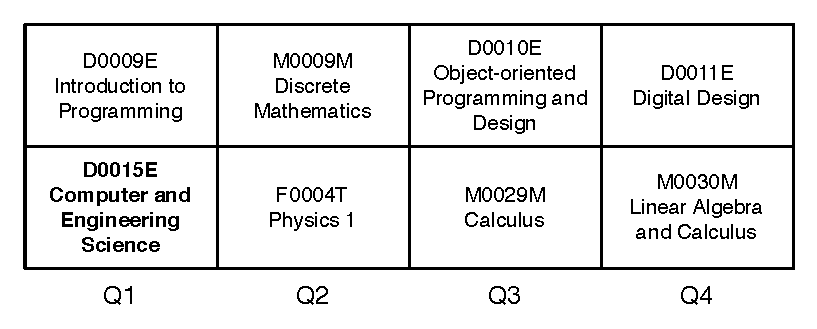
\includegraphics[width=\columnwidth]{year-one}
  \caption{Courses in year 1 and the order in which they are given. Q1, the first quarter 
                of study, starts in September, while Q4 ends in June. (D0015E is the course we 
                present in this paper.)}
  \label{fig:year-one}
\end{figure} 
The first semester was remade into containing courses on programming, an introduction, Discrete Mathematics, and Physics. 
Since students increasingly had such trouble with the Engineering Mathematics the idea was also to have the physics course, in essence classical mechanics, act like a warm-up mathematics course before reaching the Engineering Mathematics. Discrete Mathematics is – of course – a mathematics course, but one of more interest and direct use for CSE students.

The second change was that among the courses in this new CSE-early sequence, a new introductory course -- the main subject of this paper -- was added to give students an overview of the field of Computer and Engineering Science, motivate them, and prepare them technically, theoretically, and practically for the years to come and ultimately their carriers afterwards. 
It is beyond the scope of this paper to go into detail about the changes in the curriculum, how courses were re-arranged, and the reasons thereof. This paper is mainly concerned with the new course. 

\section{Course description}

The course, known as \emph{D0015E Computer and Engineering Science}~\cite{d0015e}, earns the student 7.5 ECTS\footnote{The \emph{European Credit Transfer and Accumulation System}~\cite{ects} aims to harmonize higher educations in Europe.} credits once completed. The course is given in Quarter 1, a roughly 10 week long period that starts in September, and designed so that the intended student spends a total of 200 hours studying in class and at home\footnote{One week of full-time study amounts to 40 hours and grants the successful student 1.5 ECTS credit. Students normally take two courses in parallel, studying 20 hours per week in each course.}~(Fig.~\ref{fig:year-one}). 

The course is part of our MSc degree program in Computer Science and Engineering, which is officially accredited under public Swedish law~\cite{hogskole} and highly inspired by the ACM/IEEE Curricula Recommendations~\cite{acm}. In the Fall of 2012, 62 students enrolled, which is a typical class size in the School of Engineering at our university. 

\subsection{Entry requirements}
Apart from general requirements regarding on what level an applicant must master Swedish, English, and Mathematics to at all enroll at a Swedish university, engineering students are required to have a substantially stronger background in Mathematics and Natural Sciences. In practice, the largest obstacle for students interested in applying is the Mathematics requirement. 

Being a first-year course, D0015E naturally has the same requirements. One should, however, note that although many students do also have a background in programming and other engineering related subjects, no such background is formally required. 
The youngest, and typical, applicant is 18 years old, and have been schooled for 12 years prior to applying. 

\subsection{Course aim}
The course aims to provide an understanding of the vast area of CSE and its role in the modern Information Society. This is done in several dimensions. For instance, its relation to Engineering Science and how it relates to and is used in business and academia. Integral parts of the course also focus in on practical problem solving and small engineering tasks where solutions are built using a combination of computers, electronics, and software. 
To be precise, after the course, the successful student
\begin{itemize}
  \item can define the area of CSE, in particular with relation to other engineering disciplines but also 
    Engineering Science in general by demonstrating an ability to integrate knowledge critically and 
    systematically; 

  \item is able to solve small technical problems using computers, and do so based on proven experience 
    rather than theory and formal analysis;

  \item can identify and handle computer components, programs, and common computer equipment, in 
    order to change the performance and function of a computer;

  \item knows about the main history of the area of CSE and can discuss the consequence the area has on 
    the development of modern technology, sustainability, integrity, the equality of opportunity between 
    women and men, and internationalization (globalization) by demonstrating an ability to make 
    assessments informed by relevant disciplinary, social and ethical aspects;

  \item can account for how engineers with a degree in the area of CSE work, what their typical work
    tasks are and what methods they use in research, development, and administration, and show 
    insight into current research and development work;

  \item is familiar with and can make use of modern computer-based technology for both spoken and
    written communication and collaboration over computer networks, and demonstrate a capacity for 
    teamwork and collaboration with various constellations;

  \item is able to independently find scientific information, and use such information correctly and 
    objectively,

  \item can plan and use appropriate methods to complete his/her own studies as well as advanced tasks 
    within predetermined parameters for a successful academic career within the broad area of CSE.
\end{itemize}

\subsection{Contents}

The course consists of a multifaceted study of CSE as a subject area of its own, its history, distinctive character, and artifacts. These are theoretical artifacts like (formal) languages, models, computational problems, instances, and solutions as well as physical artifacts like computer programs, digital media, and electronics. In broad terms, the area is contrasted with Engineering Science in general, that is areas directly concerned with matter and physical building materials rather than instructions and computational devices. 

The modules introduce to the students a number of problems and questions. Some of these are investigative in nature while others involve problem solving with computers or pen and paper. Computers and various software are used throughout the course. All problems or questions more or less highlight various aspects of the area of CSE as well as Engineering Science in general, and are carried out in connection with on-going research projects at the department. 

The students are also introduced to some useful tools, both technical and non-technical, handy not only during their years at the university but also as graduated engineers. They are taught, for instance, how to work in teams, give presentations, and perform interviews. Moreover, they get useful advise on techniques that improve their own studies, how they can get  information from various sources and report scientific work.

\subsection{Structure} \label{sec:modules}

The content of the course is divided into 12 separate \emph{modules} labeled A-L. Each module is centered around a topic of its own, and is examined separately. These modules form two, although only loosey connected, parallel tracks~(Fig.~\ref{fig:moment-med-pilar}). 

The first has as its theme \emph{languages}, as in ``formal languages for instructions''. It consists of the modules C, D, F, H, and J and introduce UNIX, \LaTeX, HTML~\cite{html}, Alice, and C~\cite{Kernighan:1978:CPL:7519}~(which is used to program Arduino boards).

The second track is structured around \emph{time} - the past, now, and the future. This track starts with a module on history~(E), goes on to current research performed at the department~(G) and  vital areas of research~(I), and ends with the future~(K), as well as it can be predicted right now, and a glimpse of the life of the professional engineer~(L) - the future of the majority of the students. 

\begin{figure}[!t]
  \centering
  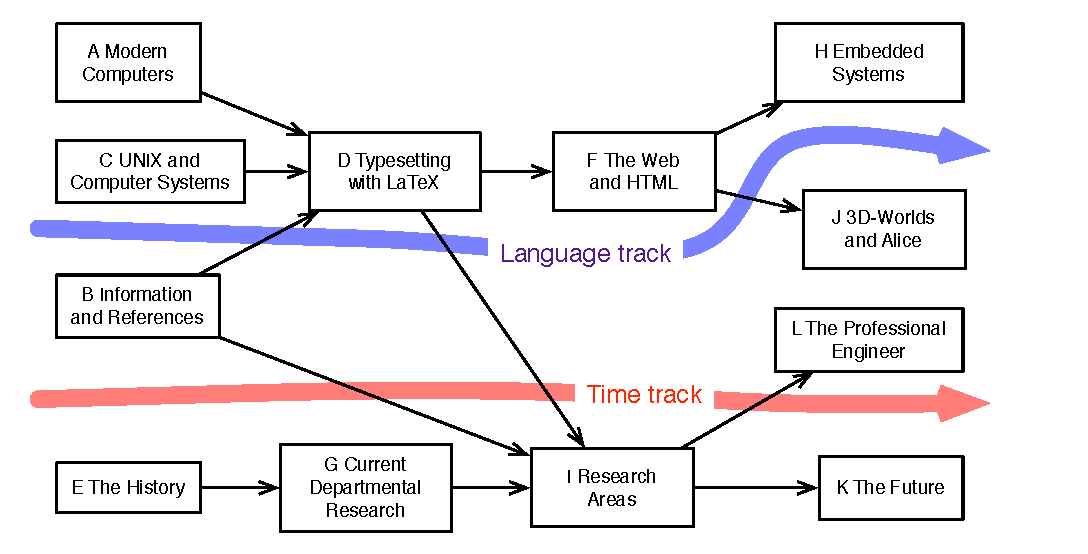
\includegraphics[width=\columnwidth]{moment-med-pilar}
  \caption{Dependencies among the course modules and the two major tracks \emph{(Formal) Languages} and \emph{Time}. }
  \label{fig:moment-med-pilar}
\end{figure}

Below we list and describe each module. One should keep in mind, while reading the list, that the course is shallow in the sense that we do not go deep into theory and analysis in the modules. There is simply no room to squeeze in what would take several years of study into the course. On the other hand, this works fine and is sufficient because our goal is (merely) to  motivate and prepare for future studies.

\subsubsection{Module A -- Modern Computers} In this module students learn about the major components that can be found in modern computers like the CPU, the mother board, cards (graphics and network), primary memory, external storage units (hard disks, DVD-readers, SSD devices, USB memory sticks etc), power units, common connectors, cords etc. In a theory part, they learn their function and are questioned orally. Then, in a practical part, they work in groups and disassemble a computer into its parts and open up components. (For this purpose, we keep a stash of old and broken hard disks and media readers through-out the year, and let the students break them before they are trashed.)

\subsubsection{Module B - Information and References} This takes place in the university library and under the guidance of experienced librarians. Students are taught how to search for and retrieve trustworthy and peer-reviewed information -- not just google for it as so many do -- and use such information in a honest way in their own work. They are also informed about the rules concerning Academic Honesty. The module contains a test that is taken on-line in an LMS~\cite{fronter}. 

\subsubsection{Module C – UNIX and Computer Systems} While all students are very tech-savvy, this module introduces something new to many: The operating system UNIX and low-level control of a computer via a command line interface. We cover commands for handling files, navigating file systems, and controlling processes but leave out more advanced topics like shell programming and system configuration. For most part of the course, although UNIX (or, in practice, Linux~\cite{siever2009linux}) might run ``under the hood'', students use computers via one of the well-known window-based graphical user interfaces. 

To pass, students first must write up experiences of their first week of study in a short document, convert it to pdf, and email it in from their university email account. Then they must complete a set of command tasks and document them with the UNIX command \texttt{script}. 

\subsubsection{Module D – Typesetting with \LaTeX} Here students learn the basics about how to typeset documents with \LaTeX. We go through the most common commands and environments ranging from overall document structure to details in mathematical formulas. The idea is to give the students the same academic typesetting tool as their professors, as well as to expose them to a formal (artificial) language with rigorous syntactic rules and semantics that resembles a programming language\footnote{\TeX, and (of course) also \LaTeX, is known to be Turing complete(!)}. 

The examination has two parts. First, students are to  produce a \LaTeX-document identical to a master provided by their instructor. Then, their task is to complete and typeset a given (hand-written) solution to a high school mathematics problem. 

\subsubsection{Module E – The History} As the name suggests, this module covers -- in a very broad sense -- the history behind the IT revolution and modern engineering. Starting with pre-historic inventions like writing and alphabets we leap through the centuries while relating new technologies to human need and the development of society. At the end, we reach the age of electricity, mass production, computers, nuclear war, space explorations, the internet, gene technology, mobile phones, and much more. The module ends with a written test. 

\subsubsection{Module F – The Web and HTML} Here, the students are introduced to another formal language: Hyper-Text Markup Language (HTML). They are also taught the basics about the Web. Using a given set of tags, the task is here to produce a detailed webpage describing the organization and function of our university. 

\subsubsection{Module G – Current Departmental Research} In this module students interview research groups at the department about their research projects, and present their findings to the class in a conference-like setting. To do so they are taught how to prepare an interview, carry it out, documenting the result, and presenting it to the class. 

\subsubsection{Module H - Embedded Systems} Most computers are embedded and this module introduces the concept of embedded systems in the form of Arduino units that the students get to experiment with. This experimentation entails both hands-on wiring of electronic components on a board and programming different functionalities  (using a simple subset of the programming language C). This is known as \emph{physical programming}, as the system normally causes some noticeable effect. To pass, the students must complete a set of lab assignments. 

\subsubsection{Module I – Research Areas} In an attempt to give further insight into our research, and bring the students closer to the department, three professors give talks about their research areas. After each talk, the students write a short, but proper, report on a topic given by the professors. They must do so using \LaTeX\  and on their own over a period of two weeks. 

\subsubsection{Module J - 3D-Worlds and Alice } Alice is a graphical programming system where programs are constructed to a large degree without typing. Alice is known for rapidly introducing someone to the ideas behind programming without having to go through the hassle of learning an old-fashioned programming language (which these students, of course, also eventually get to do).  

Here students get the task to make up a 3D-world of their liking, and write instructions that describe what should happen in these worlds. 

\subsubsection{Module K – The Future} This is a group activity in which students investigate some given sources in the literature on likely future developments in the field of Computer and Engineering Science. Findings are reported back to the class in a presentation. 
 
\subsubsection{Module L – The Professional Engineer} Here, finally, the students go on study visits to companies and meet with professional engineers. Based on these visits, the students write up their observations in the form of a short report. 

\begin{figure}[!t]
  \centering
  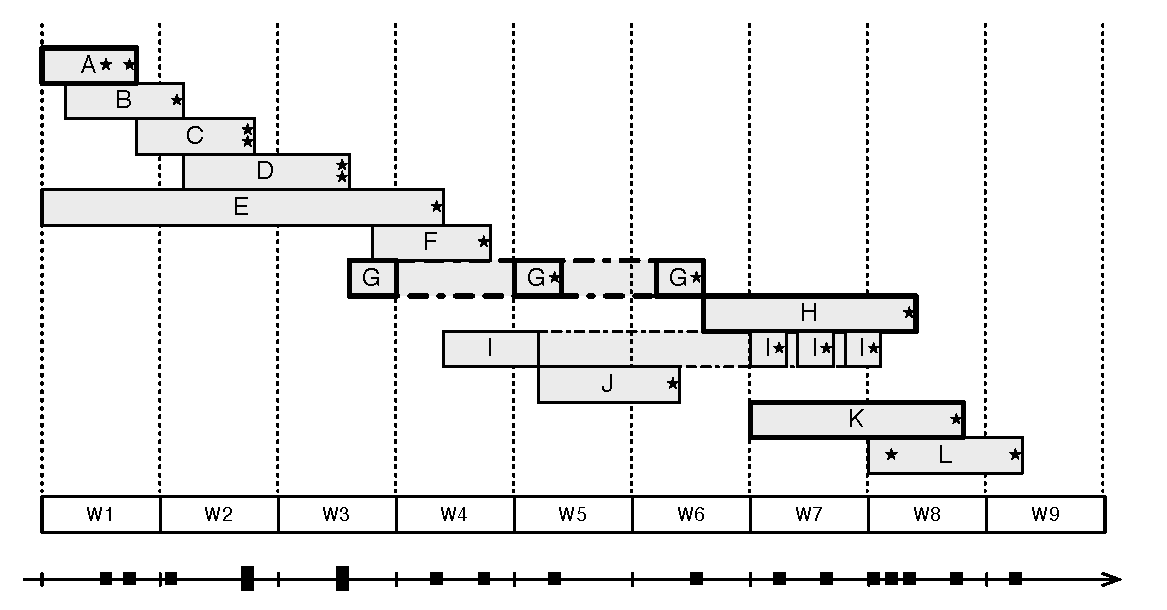
\includegraphics[width=\columnwidth]{timetable}
  \caption{A sketch of the timetable from W1 to W9, week 1 of study to week 9. Rectangles stand for modules, labeled A-L as listed in Section~\ref{sec:modules}. Stars indicate deadlines of examinations. Stars have also been projected down to black squares on the time-axis below the diagram in order to more clearly show the continuous nature of the examination that takes place during the course. Thick frames denote modules in which students work in groups.}
  \label{fig:timetable}
\end{figure}

\subsection{Realization}

Although modules are separate as far as their contents is concerned, at any given instance of time, two, and often even three, of them are simultaneously going on~(Fig.~\ref{fig:timetable}). This is intentional in order to have students plan their work on the various tasks and problems themselves in a diligent manner. 

The course is taught via lectures using AV-equipment (not writing on blackboards), educational study visits and field trips, lab assignments, writing assignments, and project work. Students also take active part in presentation, feedback, performing interviews, and interacting in (and between) groups they have been assigned to. 

The teaching is based on \emph{Constructivism}~(see, for instance, Biggs~\cite{biggs-96}), where the idea is that students construct their own understanding and knowledge of the world, through experiencing things and reflecting on those experiences, \emph{Active Learning}~\cite{BonwellE91} but with (passive) guidance first and (active) practice after that, and \emph{Inductive Learning}~\cite{Prince06inductiveteaching}. The actual instruction is inspired by \emph{Visible Learning}~\cite{hattie2009visible} in that the instructor, for instance, a) defines clear goals and criteria for achieving these goals, b) is clear about organization, explanations, examples, procedures, and assessments, and c) builds honest and trustful relations to the students by respecting their different backgrounds, listening to them, showing empathy and attention. The idea is that the student's confidence in the instructor creates a feeling of security, and that this leads to better results. 

Each module starts with one lecture in which the instructor introduces the topic of the module. Then, students start working on the tasks, module E on the history being the exception in that it instead contains some additional lectures. In module H on Embedded Systems, for example, there are a number of lab assignments to carry out. For this purpose, students are divided up into groups of three people and lent a box containing an Arduino board together with some electronic components. It is then up to the groups to organize their work with the assignments either on their own at home or on certain scheduled lab sessions, when an instructor is also present (most do the latter). During lab sessions, students build small electronic circuits that they program, and have them checked. Guided by feedback from the instructor, they improve their circuits, in case they do not meet expectation, until they have gotten everything right. There is also an assignment in which it is up to the group to also come up with what to do (within reason) and then do that. 
Students build technical solutions in this manner also in modules C, D, F, and J. In contrast, G, I, K, and L are similar in that students are asked to gather information on their own and synthesize it. However, while students give presentations in G and K they write reports in I and L. 

To aid the students in their work, and their planning, a publicly available course webpage~\cite{web-d0015e} is maintained by the instructor. This page serves as a connection point and information central for the students. It contains slides, instructions, deadlines, extra material, and various links to useful resources. This web page, together with a book on history~\cite{Sundin06} and some unpublished material written by the instructor, makes up the course literature. 

\subsection{Examination}

\begin{table}[!t]
  \centering
  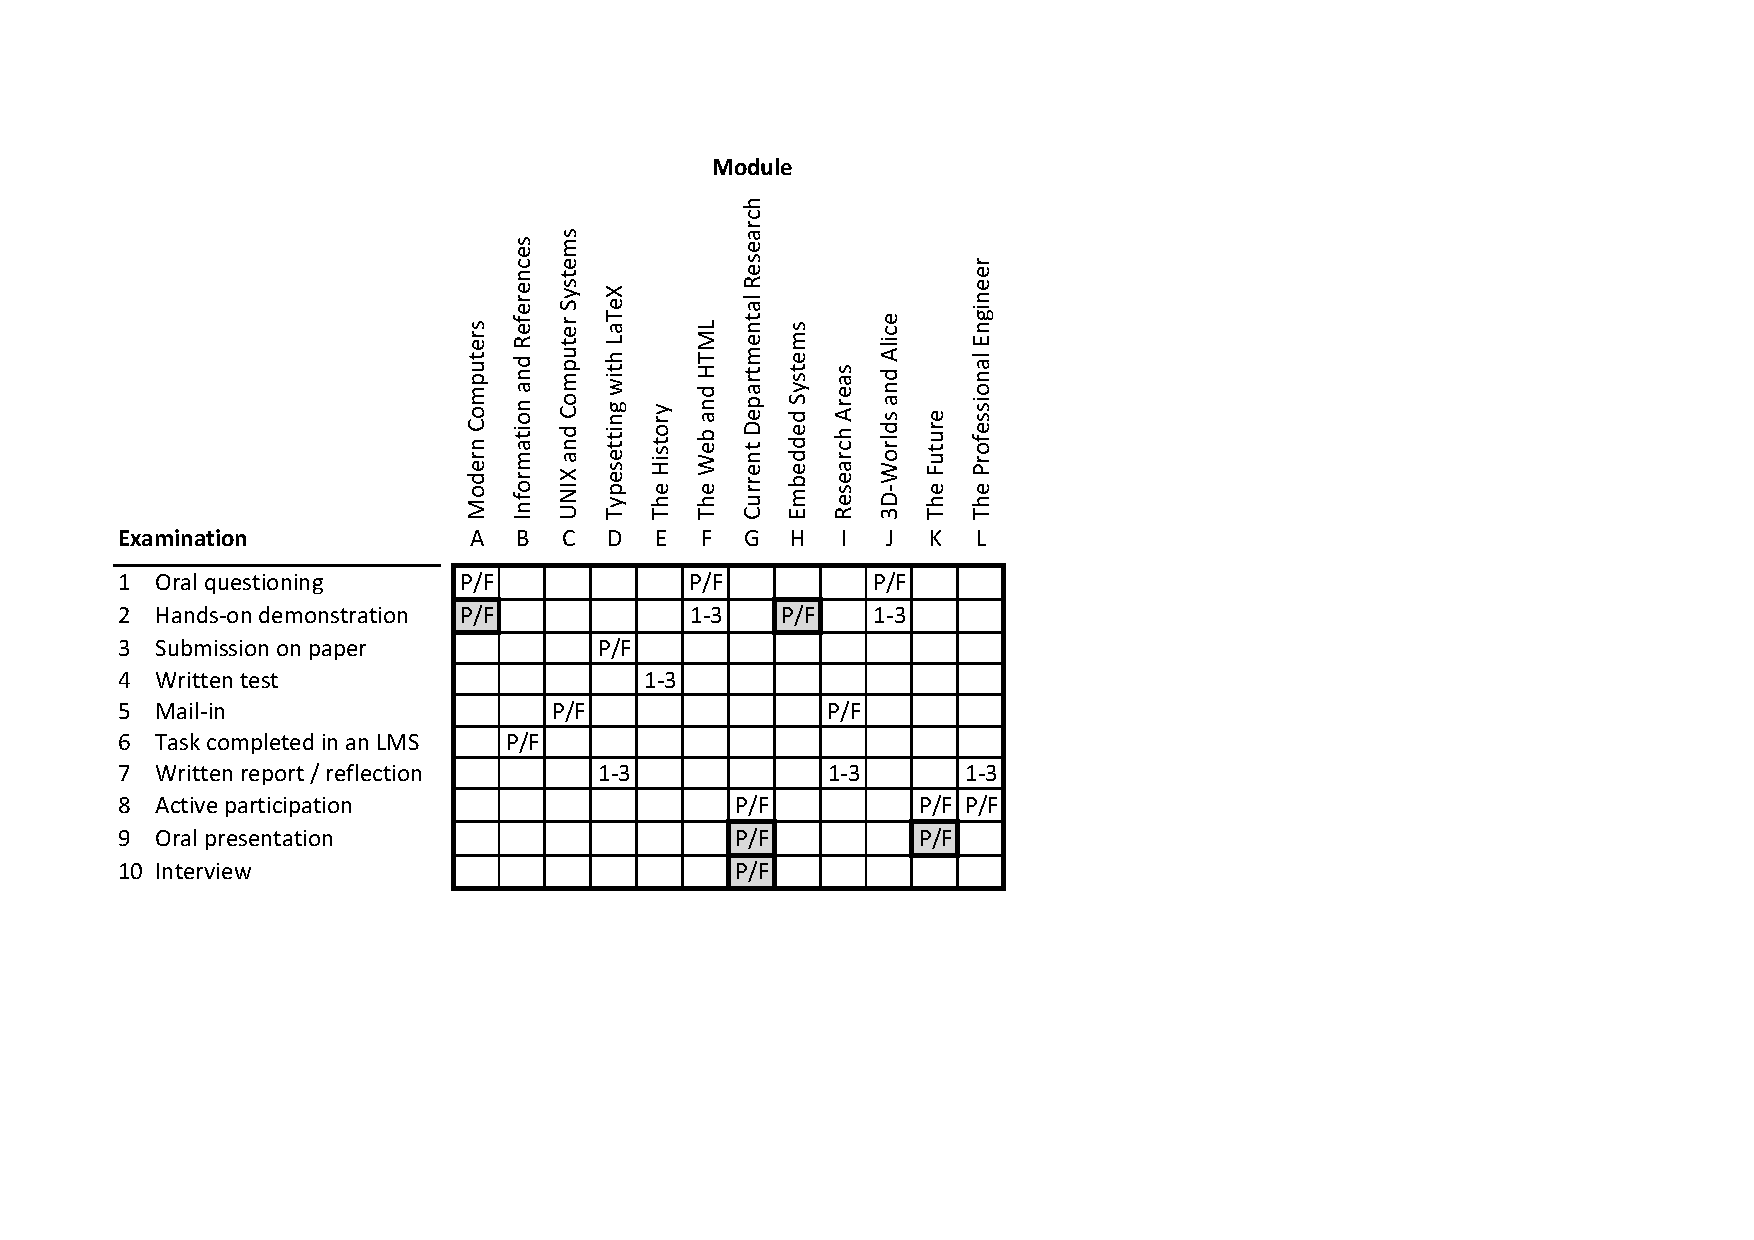
\includegraphics[width=\columnwidth]{examination}
  \caption{Kinds of examinations and ways of grading.}
  \label{fig:examination}
\end{table}

The examination is continuous throughout the course. Fig.~\ref{fig:timetable} shows the distribution of the deadlines of examinations over time in a ``Gantt chart''. In this chart, a rectangle corresponds to a module (identified by the letter). Rectangles are laid out horizontally in time-order going from left to right starting with modules A and E in Week~1 of study~(W1), and ending with module L in Week~9~(W9). While module A starts and ends in the first week, module E goes on into Week~4. Each star denotes a deadline. The downward projections of stars onto small black boxes on the time-axis below the Gantt chart is provided to more clearly visualize the continuous nature of the examinations. 

The methods of examination are deliberately chosen among those that are common within our School of Engineering such as written tests, reports, lab work and demonstrations, and conference-like oral presentations of findings to the class~(Table~\ref{fig:examination}). 
The methods of examination varies throughout the course to prepare students for courses to come. In addition, participation on presentations, field trips, visits and other joint activities is mandatory. 

\begin{table*}[!t]
  \centering
  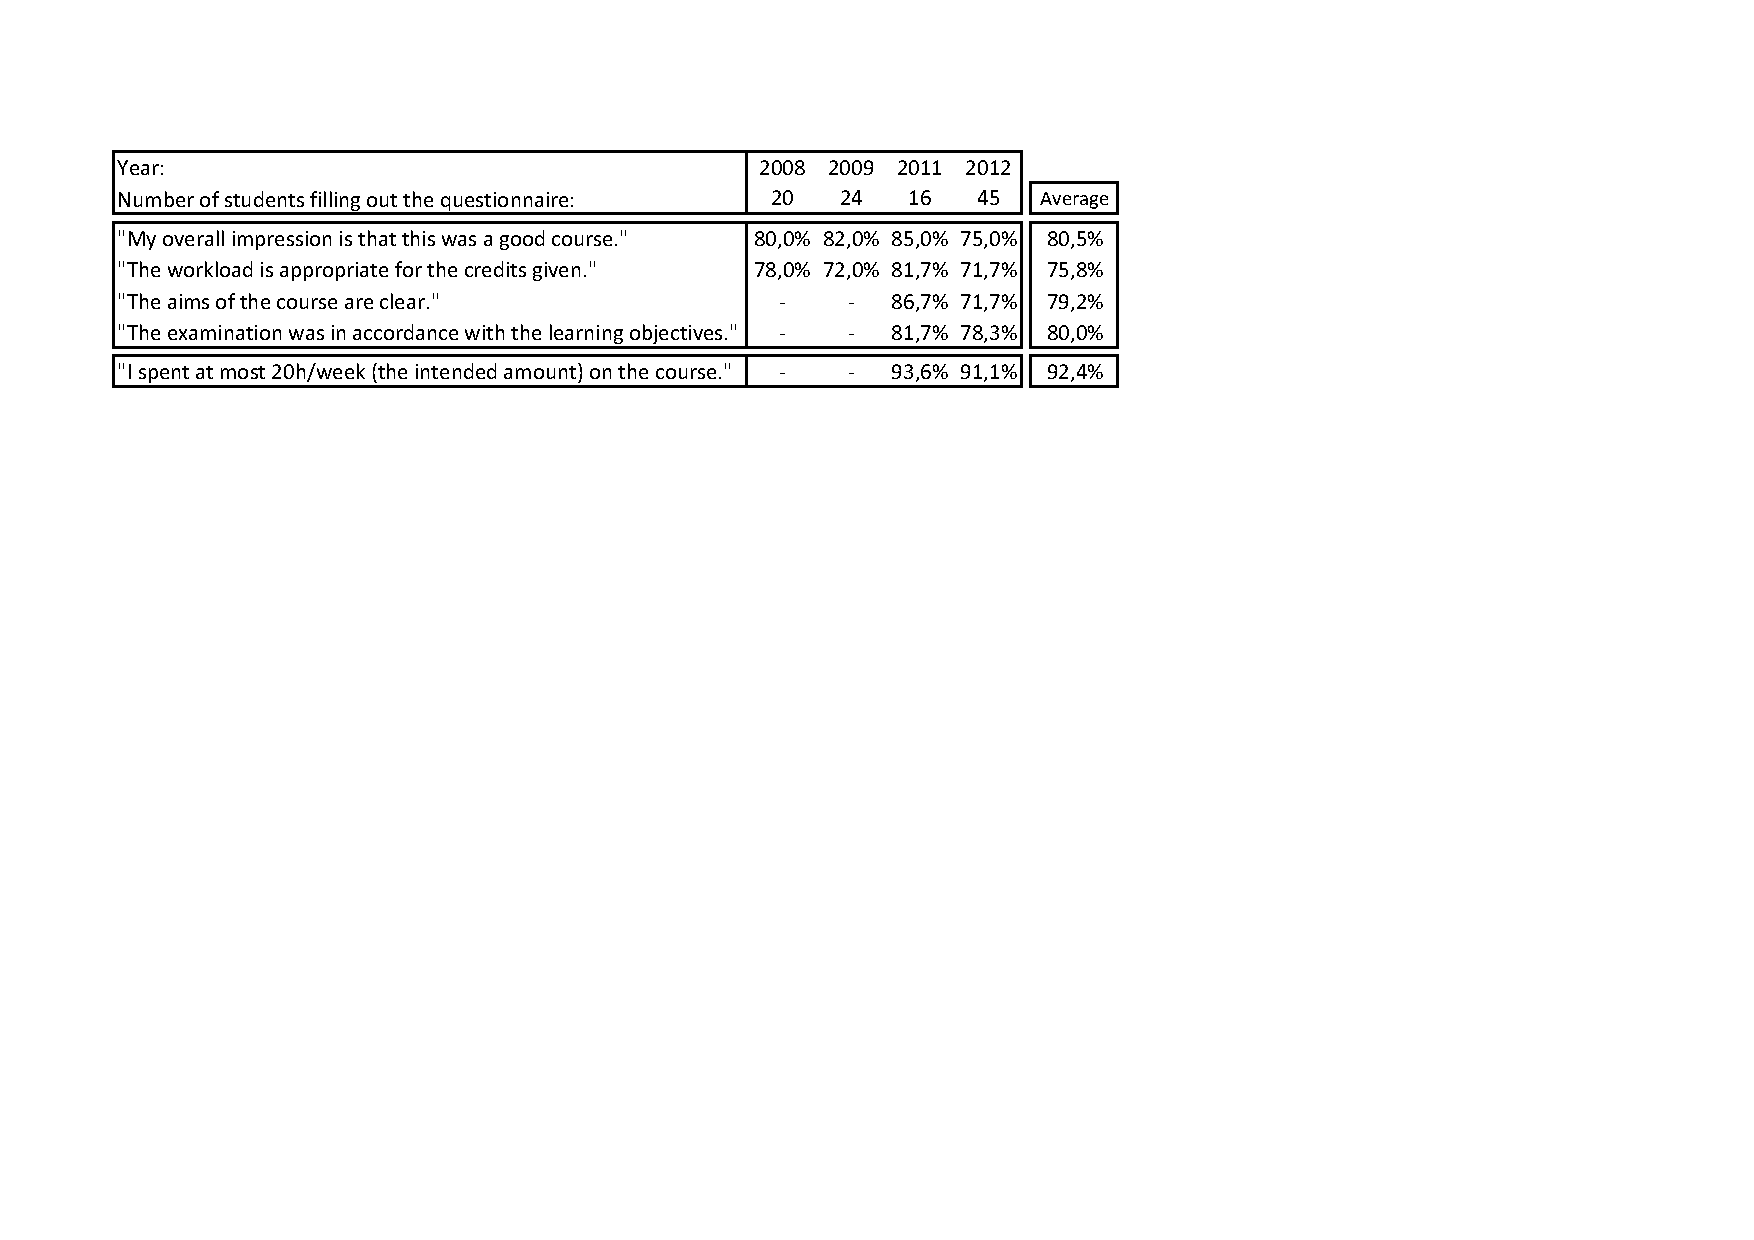
\includegraphics[width=0.65\textwidth]{course-eval}
  \caption[Statistics from questionnaires.]{Statistics from questionnaires\footnote{}.}
  \label{fig:course-eval}
\end{table*}

\subsection{Grading}

Each module has one or more examinations each of which is graded. Although some problems require students to work together in groups, and be collectively examined as a group~(shaded in Table~\ref{fig:examination}), all grades are set individually. Some examinations only give as result passed or failed while some individual examinations earn the student that pass a numerical score ranging from 1 (lowest) to 3 (highest, best). Table~\ref{fig:examination} also summarizes the two forms of grading done. Here, ``P/F'' means ``Pass or Fail'', and ``1-3'' means the grading results in a score. The final grade on the course is calculated from the scores obtained on the individual examinations only. To pass the course, however, a student must pass all examinations, not only those that give numerical scores. 

\footnotetext{Data from 2010 is unfortunately missing. The reason data is missing in 2008 and 2009 is because in these years the questionnaires were shorter and did not contain the same questions as they do now.} 

\section{Evaluation}

\begin{table}[!t]
  \centering
  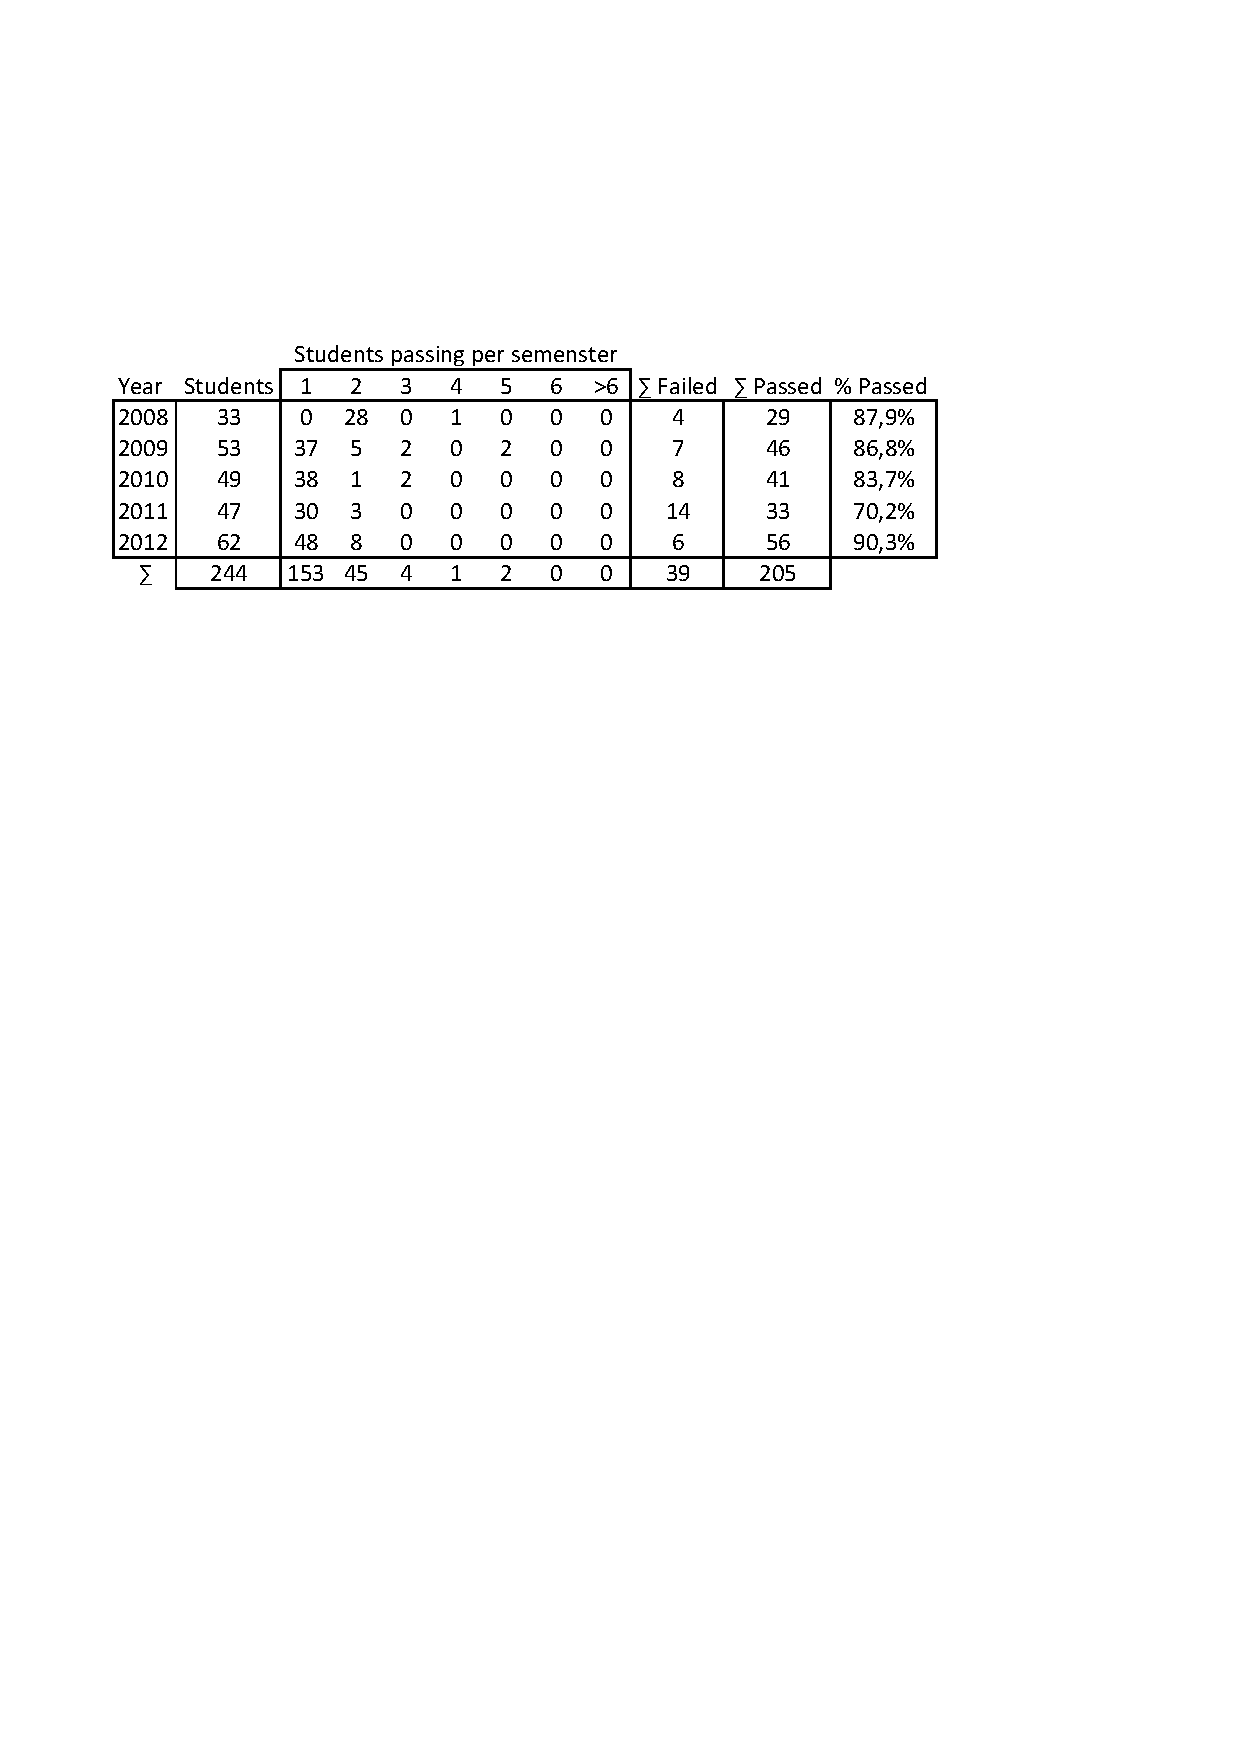
\includegraphics[width=\columnwidth]{passed}
  \caption{Number of students that pass the course and when they do so.}
  \label{fig:passed}
\end{table}

To evaluate the course we have looked at three dimensions: The course itself, effects on the educational program it belongs to, and other effects. Regarding the course itself we have used a) summaries of feedback given on questionnaire-based evaluations all students fill out directly after the course~(Table~\ref{fig:course-eval}), b) protocols from meetings with the educational board at the department, and c) official statistics over the number of students that pass the course and when they do so~(Table~\ref{fig:passed}). 

The questionnaires contain many questions and we choose here to only include results on five general ones, listed in~Table~\ref{fig:course-eval}, that relate to the overall function of the course. As they are based on answers not only from students that have passed, but also all that had failed or were not yet done at the time the questionnaire-based survey was conducted, the numbers are very high compared to many other courses. Despite the high workload experienced by almost 25\% of the students, still $92.4\%$ of them spend no more time studying than what is expected. These are signs of a course functioning well. 

In the protocols of the board, in which also higher-year students take part, the course is, in somewhat loose but still distinctive terms, deemed intense and demanding but in general good. We choose not to include them here since they only state summarized testimonies of those that are members of the board. The protocols are available from the university webpage~\cite{programrad}. 

The official statistics in Table~\ref{fig:passed} has been extracted out of the university database containing student records. These numbers are also very high compared to other courses. Directly after the course (after Semester~1), $62.7\%$ of the students have passed; after the first year of study (Semesters 1 and 2), in practice just a couple of extra months, $81.1\%$ have passed. If we would disregard the first, rather turbulent, year the course was given (2008), the number of students immediately passing the course would increase to $72.5\%$. The reason $10\%-15\%$ never pass could depend on drop-outs. 
Furthermore, from student feedback given on other questions in the questionnaires than those listed in Table~\ref{fig:course-eval}, it is clear that the average student studied a bit differently in 2011.  In 2011, the average level of attendance was for instance 4\% lower than in 2012, and the amount of preparation/reading ahead before class was 9\% lower. This difference might (perhaps) explain the sudden drop in Table~\ref{fig:passed} down to $70.2\%$ that year. However, the course was given in the same way 2011 as in other years, so the reason why students studied somewhat differently in 2011 remains unclear. 
Anyhow, the overall results show that the course works well and fulfills its goals of motivating and preparing students in line with the aims of the course. 
Moreover, introductory courses, modelled and designed after the course we have described, have today also been created and included in the program in \emph{Applied Physics and Electrical Engineering} as well as the program in \emph{Space Engineering}, two other engineering programs at our department.

\section{Conclusion and discussion}

We have presented a kind of introductory course designed for first-year engineering students in our 5-year long Master of Science program in Computer Science and Engineering. Like many other introductory courses it takes a holistic approach providing students with an overview and understanding of the vast area of Computer Science and Engineering. As we have described, the course is novel in how it is divided into 12 separate modules with a total of 21 examinations in roughly 10 weeks. Despite being tough and demanding, the course works well and manages to motivate and prepare students for further studies in line with the aims of the course. 

The first batch of students in the re-made educational program (see~Section \ref{sect:back}), to which the new introductory course belongs, are soon about to graduate. This makes it possible to determine what effect, if any, the course might have on the retention rate through-out the engineering program, for instance via a study of student records. Here, a challenge is how to isolate effects caused by the course from those caused by the re-arrangement of the order in which courses are taught and other changes in the curricula. 

\section*{Acknowledgment}

The authors would like to thank Jenny Niemi, Marie-Therese Tricot, and Jonny Johansson for kindly assisting in the process of digging out statistics over 
student performance. We thank Laurynas Riliskis for introducing us to inductive learning. We also thank him and Jingsen Chen for much appreciated feedback on an earlier draft. Finally, we are grateful to three anonymous referees whose insightful comments really improved the paper. 

%\bibliographystyle{IEEEtran}
\bibliographystyle{plain}
\bibliography{paper}

\end{document}
